\chapter{Modelado analítico de la PCC \label{chap:ModeloPCC}}
\noindent Además de los sesgos que añaden el fondo y el umbral utilizado sobre la determinación de las magnitudes del factor de Fano y la energía de creación electrón hueco, la colección parcial de carga y la eficiencia de colección de carga juegan un rol fundamental en la determinación precisa de estas magnitudes. Particularmente para las mediciones de flúor y aluminio, donde la tasa de eventos es mucho menor a la que se obtuvo en los trabajos previos\cite{TesisAndi,TesisKevin,Rodrigues} con el hierro, más apreciable es el efecto de estos fenómenos.

La física detrás de ellos puede comenzar a modelarse estudiando la distancia que recorren los fotones dentro del material del sensor hasta que interactúan con él. Esta es una variable aleatoria de distribución exponencial, que viene dada por
\begin{equation*}
    f_{Z}(z) = \frac{1}{\tau_{\scaleto{X}{4pt}}}\exp(-\frac{z}{\tau_{\scaleto{X}{4pt}}})
\end{equation*}
donde $\tau_{X}$ es la longitud de atenuación, que es la distancia promedio para la cual una cantidad de fotones incidentes reduce su cantidad a una fracción de $1/e$ de la población original. Este es un valor tabulado tanto para la energía de los fotones como para el material. Para el caso del silicio, puede verse en el gráfico de la figura \ref{fig:Attenuation} la relación entre la longitud de atenuación $\tau_{\scaleto{X}{4pt}}$ y la energía de un fotón incidente. Por ejemplo, para el caso de la energía correspondiente a los rayos $X$ del flúor, $677\,\si{eV}$, se tiene que la longitud de atenuación es aproximadamente $1\,\si{\mu m}$, mientras que para los rayos $X$ del aluminio, $\sim 1500\,\si{eV}$, la longitud de atenuación ronda los $20\,\si{\mu m}$.
\begin{figure}[h]
    \centering
        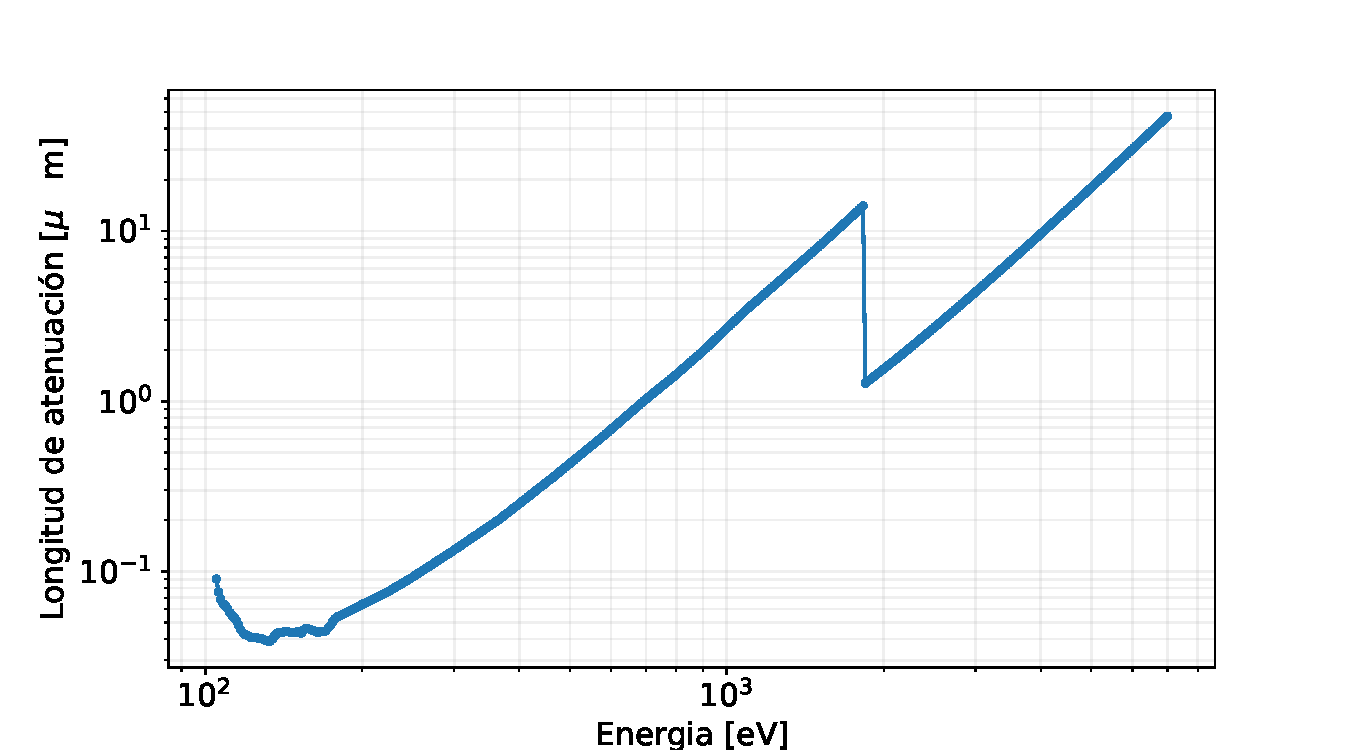
\includegraphics[scale=0.5]{Figs/AttenuationLength.pdf}
    \caption{\footnotesize{Longitud de atenuación para el silicio en función de la energía de un fotón que incide con un ángulo de $90\,^{\circ}$ sobre el material. Datos obtenidos de \textit{The Center for X-Ray Optics}\cite{AttenuationLength}.}}
    \label{fig:Attenuation}
\end{figure}

Realizaciones de la variable aleatoria de esta distribución son las diferentes distancias que puede alcanzar un fotón que penetra en el sensor hasta generar cargas por ionización.
 \ref{fig:FotoelectricoComptonPares}
\begin{figure}[h]
    \centering
        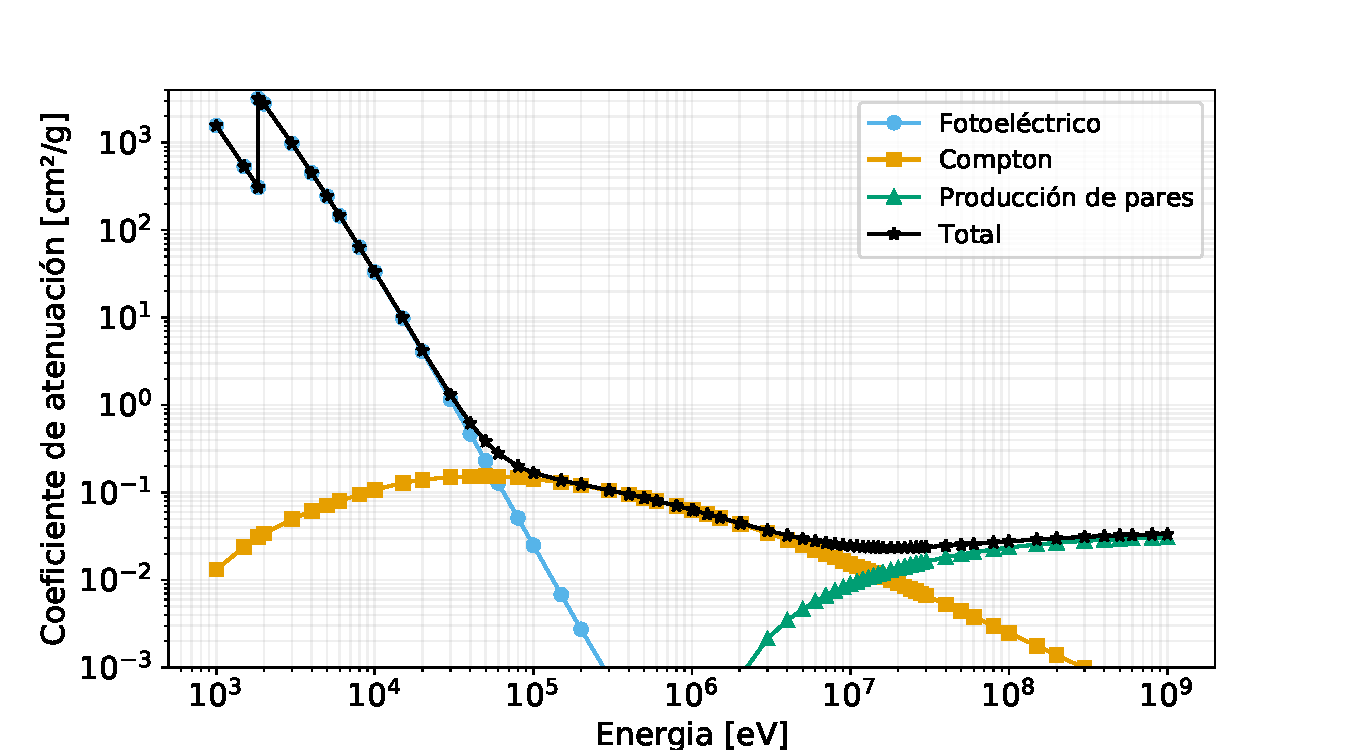
\includegraphics[scale=0.5]{Figs/FotoelectricoComptonPares_enSilicio.pdf}
    \caption{\footnotesize{Diferentes contribuciones al coefieciente de atenuación del Silicio. CHAMUYO PRELIMINAR. Cita\cite{FotoComptPar} de donde saco los datos para el plot}}
    \label{fig:FotoelectricoComptonPares}
\end{figure}
También se tiene una función para caracterizar la eficiencia de la colección de carga, tal que para una dada distancia de penetración $z$ se tiene qué porcentaje de la carga logra ser colectada y viene dada por
\begin{equation*}
    E_{ff}(z) = 1 - 
    \exp
    \left(
        -\frac{z}{\tau_{\scaleto{CCE}{4pt}}}
    \right)
\end{equation*}
donde $\tau_{CCE}$ ahora es la distancia media para la cual la cantidad de carga ionizada que sufre recombinación cae a $1/e$ del total de carga inicial. En el gráfico de la figura \ref{fig:EficienciaCC} se ven los datos obtenidos de mediciones de \textbf{DE QUÉ} y su ajuste a partir de esta función.
\begin{figure}[H]
    \centering
        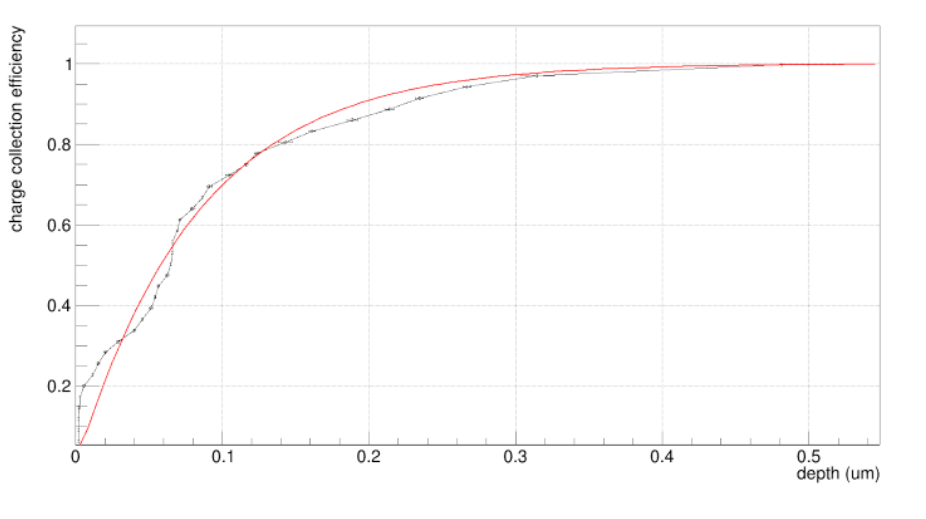
\includegraphics[scale=0.4]{pngs/CCE_plot.png}
    \caption{\footnotesize{Curva de datos y ajuste de la función de la eficiencia de la colección de carga. Se ve como el modelo ajusta muy bien a los datos obtenidos de mediciones de \textbf{DE QUÉ} y como luego de los primeros $\sim 400\,\si{nm}$ ya colecta casi el $100\,\%$ de la carga ionizada.}}
    \label{fig:EficienciaCC}
\end{figure}
Si se inyecta la variable aleatoria $z$ que viene de realizaciones de la distribución $f_{Z}$ dentro de la función $E_{ff}(z)$, mediante un cambio de variables la nueva distribución puede reescribirse como
\begin{equation*}
    f_{E_{ff}}(z) = \beta (1 - \varepsilon)^{\beta - 1}
\end{equation*}
donde se definió el parámetro $\beta$ como $\beta = \frac{\tau_{\scaleto{CCE}{2pt}}}{\tau_{\scaleto{X}{2pt}}}$. Esta es la distribución de probabilidad de colectar la carga producida por un fotón de una dada energía.

Sin embargo, para terminar de modelar todos los efectos que contribuyen a la dispersión de la carga generada por ionización en el material, hay que considerar que, además de los efectos anteriores, para una dada energía no siempre se producirán la misma cantidad de carga. Este efecto es descripto por el factor de Fano. Dado que cada proceso de ionización puede considerarse como un experimento de Bernoulli, una sucesión de interacciones puede pensarse como un fenómeno binomial. En el límite, donde la probabilidad de ionización es baja y la cantidad de veces que puede haber interacciones es muy alta, el proceso se vuelve Poissoniano. Cuando la esperanza de dicha distribución es alta (mayor a $100$ en los casos de interés en este trabajo), el límite gaussiano dado por el teorema central del límite se cumple en excelente aproximación. Con lo cual, la distribución de carga para los eventos de interés puede modelarse sin perder precisión con una distribución gaussiana. Para agregar esta última contribución al modelado del fenómeno es necesario realizar la convolución de ambas distribuciones: La distribución de probabilidad de colectar carga dada una distancia de penetración $z$ y la distribución de probabilidad de generar carga dada una energía inicial. De hacer este cálculo se obtiene la siguiente expresión
\begin{equation*}
    f_{Q_{f}}(q_{f}) = 
    \int\limits_{0}^{1}
    \frac{\beta}{\sqrt{2\pi \sigma^{2}}\varepsilon}
    \exp[%
    -\frac{(q_{f}-\varepsilon\mu)^{2}}{2\sigma^{2}\varepsilon^{2}}
    ](1-\varepsilon)^{\beta - 1}
    d\varepsilon
\end{equation*}
para la distribución teórica de carga debido a los efectos del factor de Fano y la colección parcial de carga actuando conjuntamente.

Utilizar este modelo para ajustar los picos de los histogramas de carga tiene la ventaja de que los parámetros que obtienen del ajuste, como el valor medio $\mu$ y su dispersión $\sigma$, son los valores que se obtendrían si la colección parcial de carga fuera totalmente nula. Es decir, este modelo logra obtener estas magnitudes disociando totalmente el efecto de la PCC. 


%\indent Si el detector fuera perfecto, el factor de Fano existiría igual. Este no es un problema del detector, viene del proceso de interacción en sí mismo que a la larga es un fenómeno binomial. Sin embargo, lo que sí es un problema del detector es la PCC. Un fotón interactuando con materia es un experimento Bernoulli, una serie de procesos de interacción es un fenómeno binomial y, en consecuencia, en el límite de probabilidades pequeñas y gran número de repeticiones, de Poisson. Por lo tanto, cuán lejos llega es una variable aleatoria con distribución exponencia (La distancia entre dos eventos de poisson es exponencial). Si uno quiere saber cuál es la probabilidad de que un fotón penetre una dada distancia, hay que hacer
%\begin{equation*}
%    e^{-\frac{d}{\tau}}
%\end{equation*}
%con $\tau$ es la attenuation length. La eficiencia de colección de carga viene dada por 
%\begin{equation*}
%    E_{ff}(z) = 1 - e^{-\frac{z}{\tau_{\scaleto{CEE}{2pt}}}}
%\end{equation*}
%que quiere decir que si la interacción se realizó para un dado $z_{0}$, entonces por ejemplo el $70\%$ de la carga logró ser colectada. Para $Z_{0}$ muy chico, la eficiencia es muy chica, para $z_{0}$ creciente, la eficiencia es creciente.

%Dada la variable aleatoria: Longitud penetrada hasta interactuar, tiene una distribución exponencial. Dada una energía fija, la longitud que recorre hasta interactuar no es siempre la misma, hay una aleatoria inherente. La distribución de probabilidades de este experimento es exponencial. Si por ejemplo la probabilidad de interactuar en los primeros $3\,\si{\mu m}$ es del $50\%$, la probabilidad de interactuar recién luego de recorridos $80\,\si{\mu m}$ es $10^{-14}$. Esta variable aleatoria se inyecta dentro de la función $E_{ff}(z)$: Función a la que le digo hasta donde llegó la partícula antes de interactuar y devuelve con qué eficiencia colectó la carga.

%Se tiene la energía del fotón, se genera un evento aleatorio con distribución exponencial $z_{0}$ que dice qué distancia penetró el fotón antes de interactuar. Esa realización se usa como argumento de $E_{ff}(z) \longrightarrow E_{ff}(z_{0})$. Ese cambio de variables da como resultado 
%\begin{equation*}
%    f_{E_{ff}}(z) = \beta (1 - \varepsilon)^{\beta - 1}
%\end{equation*}
%donde $\beta = \frac{\tau_{\scaleto{CCE}{3pt}}}{\tau_{\scaleto{X}{3pt}}}$. La probabilidad de recuperar la carga de un fotón de una dada energía sigue esa distribución.

%Todavía no entró el Fano. A esto hay que agregarle que además de haber una distribución de carga para la profundidad, además de haber una función que dice cuánta carga se logra colectar con esa profundidad, hay otra variable aleatoria que es cuántos electrones se ionizan cuando se interactúa, que viene de una poissoniana, pero en el límite se puede pensar como una gaussiana. Entonces, a la función anterior hay que convolucionarla con una gaussiana. El efecto de convolucionar una gaussiana con esta distribución es añadirle una cola del lado izquierdo a la gaussiana. De hacer esa convolución se obtiene
%\begin{equation*}
%     f_{Q_{f}}(q_{f}) = 
%     \int\limits_{0}^{1}
%     \frac{\beta}{\sqrt{2\pi \sigma^{2}}\varepsilon}
%     \exp[%
%     -\frac{(q_{f}-\varepsilon\mu)^{2}}{2\sigma^{2}\varepsilon^{2}}
%     ](1-\varepsilon)^{\beta - 1}
%     d\varepsilon
% \end{equation*}
%La cola que aparece a la izquierda es culpa de la PCC, debido a que hay eventos con menor carga generada debido a este fenómeno de recombinación para los eventos que suceden en los primeros micrones del detector. Del lado derecho no hay nada porque no hay un fenómeno que genere más carga de la que el proceso de ionización puede generar.
%%%%%%%%%%%%%%%%%%%%%%%%%%%%%%%%%%%%%%%%%%%%%%%%%%%%%%%%%%%%%%%%%%
%%%%%%%%%%%%%%%%%%%%%%%%%%%%%%%%%%%%%%%%%%%%%%%%%%%%%%%%%%%%%%%%%%
